%%%%%%%%%%%%%%
%% Run LaTeX on this file several times to get Table of Contents,
%% cross-references, and citations.

%% w-bktmpl.tex. Current Version: Feb 16, 2012
%%%%%%%%%%%%%%%%%%%%%%%%%%%%%%%%%%%%%%%%%%%%%%%%%%%%%%%%%%%%%%%%
%
%  Template file for
%  Wiley Book Style, Design No.: SD 001B, 7x10
%  Wiley Book Style, Design No.: SD 004B, 6x9
%
%  Prepared by Amy Hendrickson, TeXnology Inc.
%  http://www.texnology.com
%%%%%%%%%%%%%%%%%%%%%%%%%%%%%%%%%%%%%%%%%%%%%%%%%%%%%%%%%%%%%%%%

%%%%%%%%%%%%%%%%%%%%%%%%%%%%%%%%%%%%%%%%%%%%%%%%%%%%%%%%%%%%%%%%
%% Class File

%% For default 7 x 10 trim size:
%\documentclass{WileySev}

%% Or, for 6 x 9 trim size
\documentclass{WileySix}

%%%%%%%%%%%%%%%%%%%%%%%%%%%%%%%%%%%%%%%%%%%%%%%%%%%%%%%%%%%%%%%%
%% Post Script Font File

% For PostScript text
% If you have font problems, you may edit the w-bookps.sty file
% to customize the font names to match those on your system.

\usepackage{w-bookps}

%%%%%%%
%% For times math: However, this package disables bold math (!)
%% \mathbf{x} will still work, but you will not have bold math
%% in section heads or chapter titles. If you don't use math
%% in those environments, mathptmx might be a good choice.

% \usepackage{mathptmx}


%%%%%%%%%%%%%%%%%%%%%%%%%%%%%%%%%%%%%%%%%%%%%%%%%%%%%%%%%%%%%%%%
%% Graphicx.sty for Including PostScript .eps files

\usepackage{graphicx}


%%%%%%%%%%%%%%%%%%%%%%%%%%%%%%%%%%%%%%%%%%%%%%%%%%%%%%%%%%%%%%%%
%% Other packages you might want to use:

% for chapter bibliography made with BibTeX
% \usepackage{chapterbib}

% for multiple indices
% \usepackage{multind}

% for answers to problems
% \usepackage{answers}




%%%%%%%%%%%%%%%%%%%%%%%%%%%%%%%%%%%%%%%%%%%%%%%%%%%%%%%%%%%%%%%%
%% Change options here if you want:
%%
%% How many levels of section head would you like numbered?
%% 0= no section numbers, 1= section, 2= subsection, 3= subsubsection
%%==>>
\setcounter{secnumdepth}{3}

%% How many levels of section head would you like to appear in the
%% Table of Contents?
%% 0= chapter titles, 1= section titles, 2= subsection titles, 
%% 3= subsubsection titles.
%%==>>
\setcounter{tocdepth}{2}

%% Cropmarks? good for final page makeup
%% \docropmarks %% turn cropmarks on

%%%%%%%%%%%%%%%%%%%%%%%%%%%%%%%%%%%%%%%%%%%%%%%%%%%%%%%%%%%%%%%%
%% DRAFT
%
% Uncomment to get double spacing between lines, current date and time
% printed at bottom of page.
% \draft
% (If you want to keep tables from becoming double spaced also uncomment
% this):
% \renewcommand{\arraystretch}{0.6}
%%%%%%%%%%%%%%%%%%%%%%%%%%%%%%

\begin{document}

%%%%%%%%%%%%%%%%%%%%%%%%%%%%%%%%%%%%%%%%%%%%%%%%%%%%%%%%%%%%%%%%
%% Title Pages
%%
%% Wiley will provide title and copyright page, but you can make
%% your own titlepages if you'd like anyway

%% Setting up title pages, type in the appropriate names here:
\booktitle{Sistem Informasi Geografis}
\subtitle{Mengenal dan Membangun SIG}

\author{Rolly Maulana Awangga}
%\affil{Program Studi Sarjana Terapan Teknik Informatika Politeknik Pos Indonesia}
%or
%\authors{}

%% \\ will start a new line.
%% You may add \affil{} for affiliation, ie,
%\authors{Robert M. Groves\\
%\affil{Universitat de les Illes Balears}
%Floyd J. Fowler, Jr.\\
%\affil{University of New Mexico}
%}

%% Print Half Title and Title Page:
\halftitlepage
\titlepage


%%%%%%%%%%%%%%%%%%%%%%%%%%%%%%%%%%%%%%%%%%%%%%%%%%%%%%%%%%%%%%%%
%% Off Print Info

%% Add your info here:
\offprintinfo{Sistem Informasi Geografis, pre-release}{Rolly Maulana Awangga}

%% Can use \\ if title, and edition are too wide, ie,
%% \offprintinfo{Survey Methodology,\\ Second Edition}{Robert M. Groves}


%%%%%%%%%%%%%%%%%%%%%%%%%%%%%%%%%%%%%%%%%%%%%%%%%%%%%%%%%%%%%%%%
%% Copyright Page

\begin{copyrightpage}{2017}
Sistem Informasi Geografis / Rolly Maulana Awangga
\end{copyrightpage}

% Note, you must use \ to start indented lines, ie,
% 
% \begin{copyrightpage}{2004}
% Survey Methodology / Robert M. Groves . . . [et al.].
% \       p. cm.---(Wiley series in survey methodology)
% \    ``Wiley-Interscience."
% \    Includes bibliographical references and index.
% \    ISBN 0-471-48348-6 (pbk.)
% \    1. Surveys---Methodology.  2. Social 
% \  sciences---Research---Statistical methods.  I. Groves, Robert M.  II. %
% Series.\\

% HA31.2.S873 2004
% 001.4'33---dc22                                             2004044064
% \end{copyrightpage}

%%%%%%%%%%%%%%%%%%%%%%%%%%%%%%%%%%%%%%%%%%%%%%%%%%%%%%%%%%%%%%%%
%% Frontmatter >>>>>>>>>>>>>>>>

%%%%%%%%%%%%%%%%%%%%%%%%%%%%%%%%%%%%%%%%%%%%%%%%%%%%%%%%%%%%%%%%
%% Only Dedication (optional) 
%% or Contributor Page for edited books
%% before \tableofcontents

\dedication{For my family}

% ie,
%\dedication{To my parents}

%%%%%%%%%%%%%%%%%%%%%%%%%%%%%%%%%%%%%%%%%%%%%%%%%%%%%%%%%%%%%%%%
%  Contributors Page for Edited Book
%%%%%%%%%%%%%%%%%%%%%%%%%%%%%%%%%%%%%%%%%%%%%%%%%%%%%%%%%%%%%%%%

% If your book has chapters written by different authors,
% you'll need a Contributors page.

% Use \begin{contributors}...\end{contributors} and
% then enter each author with the \name{} command, followed
% by the affiliation information.

% \begin{contributors}
% \name{Masayki Abe,} Fujitsu Laboratories Ltd., Fujitsu Limited, Atsugi,
% Japan

% \name{L. A. Akers,} Center for Solid State Electronics Research, Arizona
% State University, Tempe, Arizona

% \name{G. H. Bernstein,} Department of Electrical and
% Computer Engineering, University of Notre Dame, Notre Dame, South Bend, 
% Indiana; formerly of
% Center for Solid State Electronics Research, Arizona
% State University, Tempe, Arizona 
% \end{contributors}

%%%%%%%%%%%%%%%%%%%%%%%%%%%%%%%%%%%%%%%%%%%%%%%%%%%%%%%%%%%%%%%%
\contentsinbrief %optional
\tableofcontents
% \listoffigures %optional
% \listoftables  %optional

%%%%%%%%%%%%%%%%%%%%%%%%%%%%%%%%%%%%%%%%%%%%%%%%%%%%%%%%%%%%%%%%
% Optional Foreword:

%\begin{foreword}
%text
%\end{foreword}

%%%%%%%%%%%%%%%%%%%%%%%%%%%%%%%%%%%%%%%%%%%%%%%%%%%%%%%%%%%%%%%%
% Optional Preface:

%\begin{preface}
% text
%\prefaceauthor{}
%\where{place\\
% date}
%\end{preface}

% ie,
% \begin{preface}
% This is an example preface.
% \prefaceauthor{R. K. Watts}
% \where{Durham, North Carolina\\
% September, 2004}

%%%%%%%%%%%%%%%%%%%%%%%%%%%%%%%%%%%%%%%%%%%%%%%%%%%%%%%%%%%%%%%%
% Optional Acknowledgments:

% \acknowledgments
% acknowledgment text
% \authorinitials{} % ie, I. R. S.


%%%%%%%%%%%%%%%%%%%%%%%%%%%%%%%%
%% Glossary Type of Environment:

% \begin{glossary}
% \term{<term>}{<description>}
% \end{glossary}

%%%%%%%%%%%%%%%%%%%%%%%%%%%%%%%%
% \begin{acronyms} 
% \acro{<term>}{<description>}
% \end{acronyms}

%%%%%%%%%%%%%%%%%%%%%%%%%%%%%%%%
%% In symbols environment <term> is expected to be in math mode; 
%% if not in math mode, use \term{\hbox{<term>}}

% \begin{symbols}
% \term{<math term>}{<description>}
% \term{\hbox{<non math term>}}Box used when not using a math symbol.
% \end{symbols}

%%%%%%%%%%%%%%%%%%%%%%%%%%%%%%%%
% \begin{introduction}
%\introauthor{<name>}{<affil>}
% Introduction text...
% \end{introduction}

%%%%%%%%%%%%%%%%%%%%%%%%%%%%%%%%%%%%%%%%%%%%%%%%%%%%%%%%%%%%%%%%
%% End for Front Matter, Beginning of text of book  >>>>>>>>>>>

%% Short version of title without \\ may be written in sq. brackets:

%% Optional Part :
\part[Pendahuluan]
{Pendahuluan\\ Pengantar Geospasial}

%\chapter[Pendahuluan]
%{Pengantar\\ Sistem Informasi Geografis}
%\prologue{The sheer volumne of answers can often stifle insight...The purpose
of computing\index{computing!the purpose} is insight, not numbers.}
{Hamming}

\section{Definisi}
Sistem Informasi Geografis merupakan penggalan kata dan Sistem Informasi dan Geografis. Geografis dipandang sebagai bentukan dari geospasial.
Geospasial memiliki arti geo yang berarti bumi dan spasial yang berarti ruang atau keruangan. Jadi geospasial merupakan ilmu yang mempelajari 
tata ruang dari bumi. Tata ruang melingkupi letak suatu titik di bumi baik itu letak kota, provinsi atau negara. Tata ruang juga menyajikan gambaran dari ruang tersebut yang disebut dengan ilmu kartografi atau sering disebut sebagai ilmu pembuatan peta\cite{IEEEhowto:IEEEtranpage}.

\section{Sejarah Peta}
Perkembangan peta dunia tidak luput dari para ahli geografi dan kartografi. Peta dunia yang populer pada saat ini merupkan kontribusi dari para 
pembuat peta sebelumnya

\subsection{Ptolemy's}
Ptolemy's diduga membuat peta pada abad ke 2


\subsection{Muhammad al-Idrisi}
Seorang ahli geografi dan kartografi Muhammad al-Idrisi membuat peta dunia pada abad ke 11

\begin{figure}[ht]

\centerline{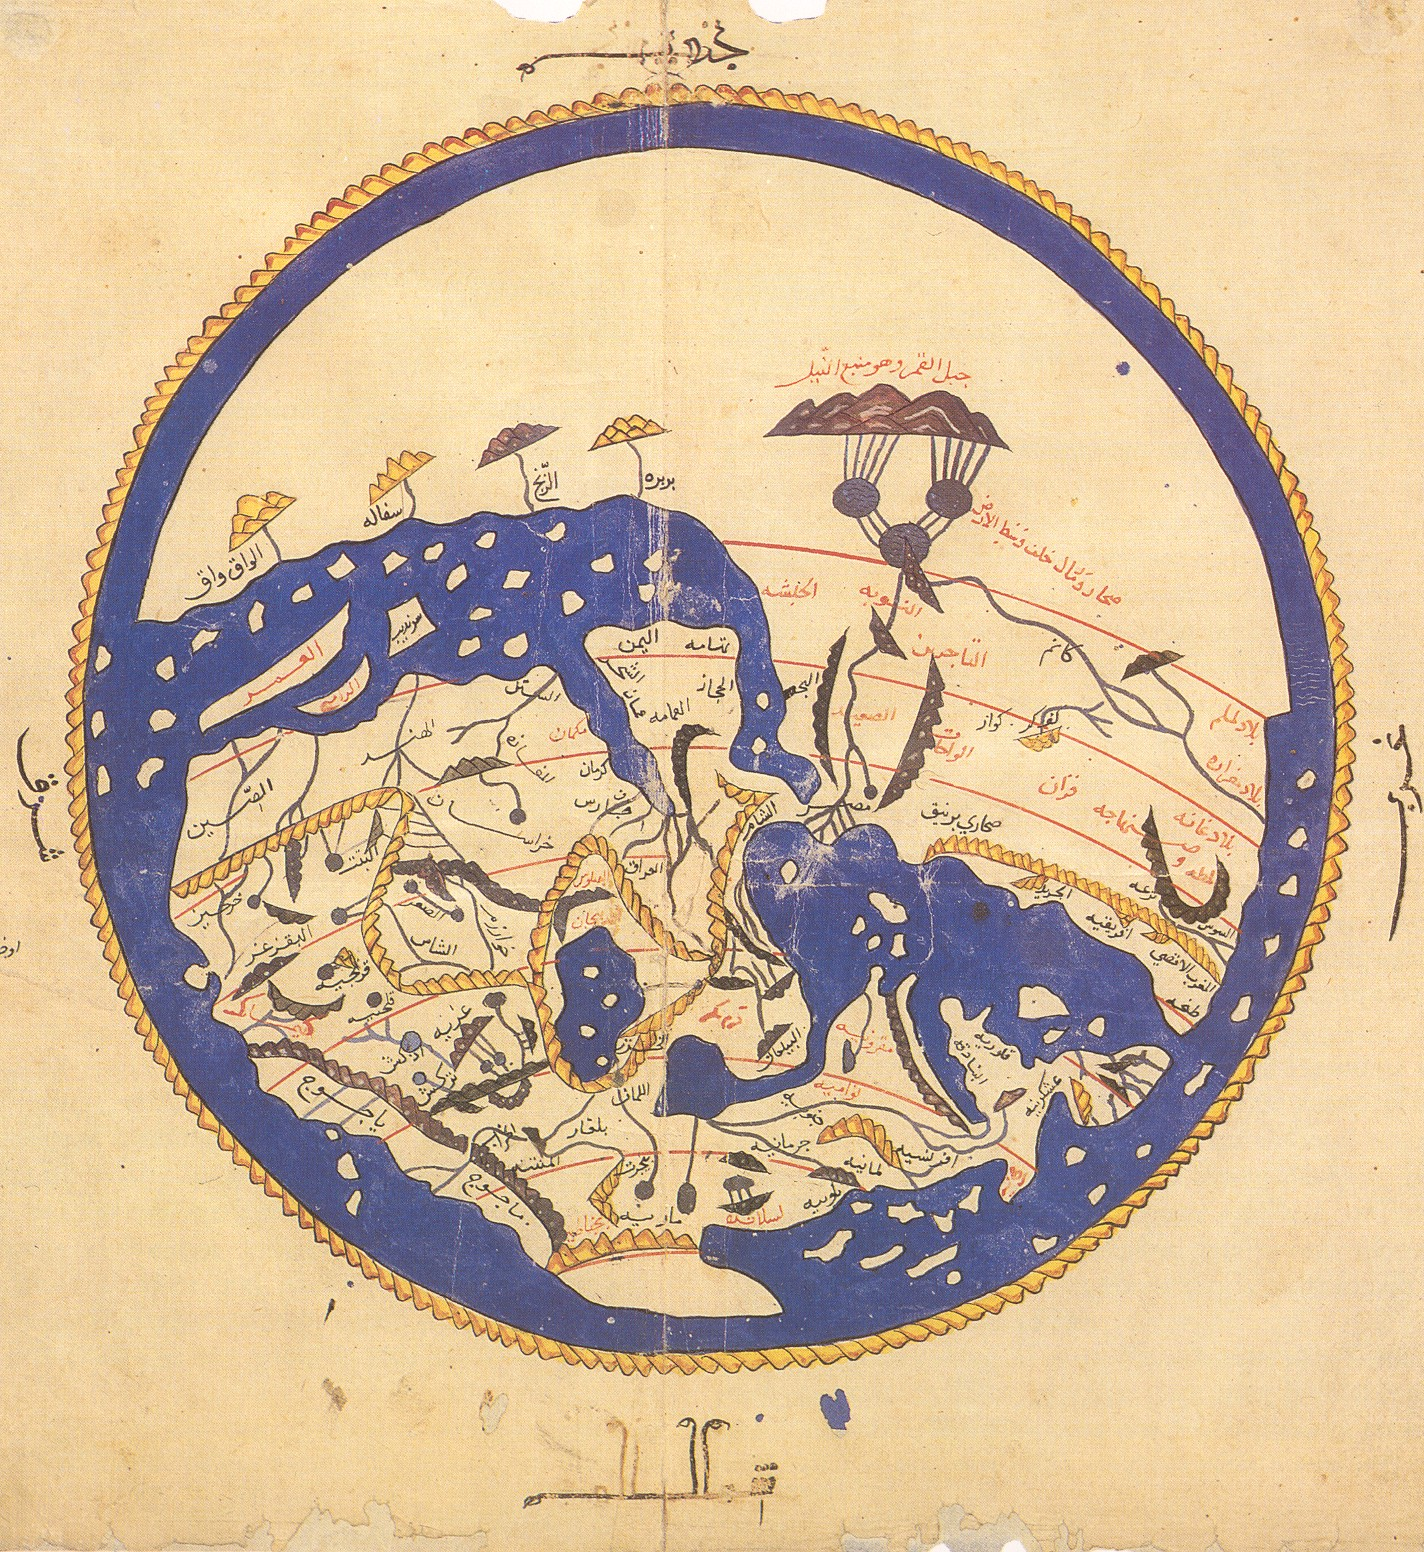
\includegraphics[width=1\textwidth]{figures/petaduniaalid.JPG}}
\caption{Gambaran pengantar peta dunia karya al-Idrisi tahun 1154.}
\end{figure}

\begin{figure}[ht]
	\centerline{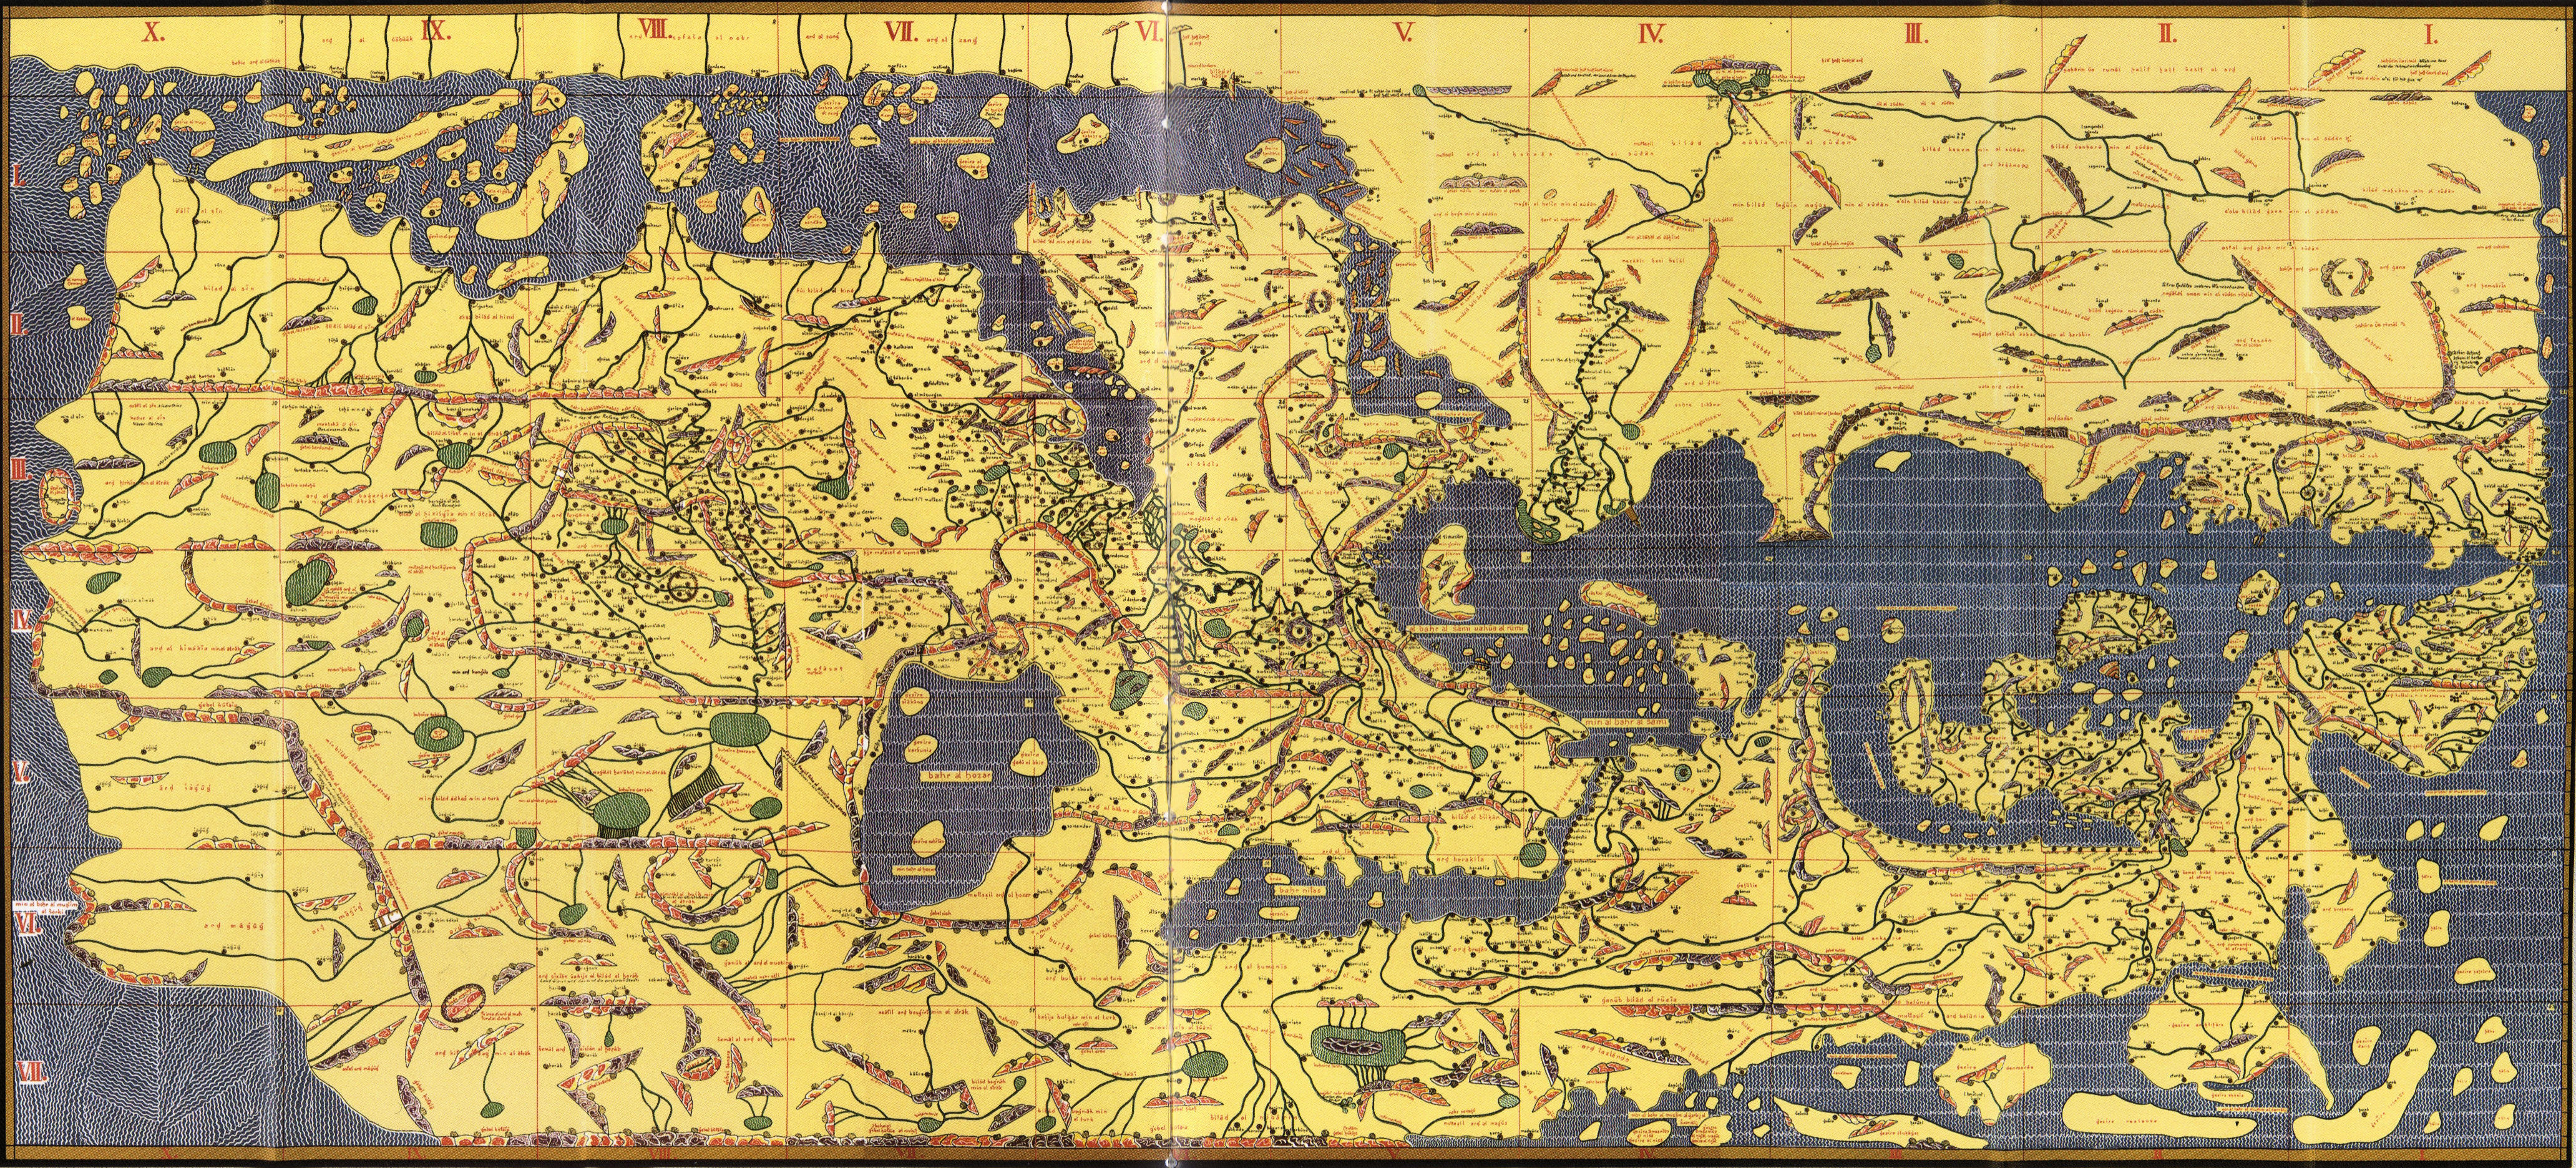
\includegraphics[width=1\textwidth]{figures/TabulaRogeriana.jpg}}
\vskip2pt
\caption{Tabula Rogeriana digambar oleh Al-Idrisi pada tahun 1154 untuk Raja Normandia Roger II dari Sisilia, setelah delapan menetap di istananya, di mana dia bekerja untuk penjelasan dan ilustrasi peta.}
\end{figure}

\section{Penentuan Kordinat}
Kordinat digunakan untuk mengacu sebuah titik lokasi di muka bumi, adapun beberapa jenis standar kordinat yang digunakan adalah.

\subsection{Kordinat Internasional}
Kordinat internasional dikenal dengan long dan lat.


\subsection{Kordinat Indonesia}
Masih ingatkah pelajaran geografi tentang letak Indonesia? maka kita bisa melihat jawaban tersebut dalam kordinat berbahasa indonesia.



\chapter[Pendahuluan]
{Pendahuluan\\ definisi}
% kelompok definisi
% ariana setiawan (1154042)
% idang mawardi (1154084)
% arya niken manalu (1154080)
% M. Arya Sikumbang (1154075)
% r rifa fauzi komara (1154089)
% Andi Tenri Wali (1154013)

\section{Definisi GIS (GEOGRAPHICS INFORMATION SYSTEM)}
Geographical information system (GIS) adalah sebuah komputer yang berbasis sistem
informasi digunakan untuk memberikan informasi bentuk digital dan analisa terhadap 
permukaan geografi bumi.

\subsection{Pemahaman pada Geographics Information System GIS}
Dimana GIS merupakan pemahaman dari, sebagai berikut:
\begin{enumerate}
\item Geography

Dimana GIS dibangun berdasarkan pada istilah‘geografi’ atau ‘spasial’.
Object mengacu pada spesifikasi lokasi dalam suatu tempat/ruang. Objek dapat berupa fisik,
budaya ataupun ekonomi alamiah. Penampakan yang seperti ini ditampilkan pada suatu peta yang 
digunakan untuk memberikan gambaran yang lebih representatif dari spasial dari suatu objek.
sesuai dengan kenyataannya yang di bumi. Dimana simbol, warna dan gaya garis digunakan sebagai
perwakilan dari setiap spasial yang berbeda pada peta dua dimensi.
Pada gambar \ref{dataspasial} dijelaskan bahwa data spasial berikut berupa 
titik, garis, poligon (2-D) dan permukaan (3-D).

\begin{figure}[ht]
	\centerline{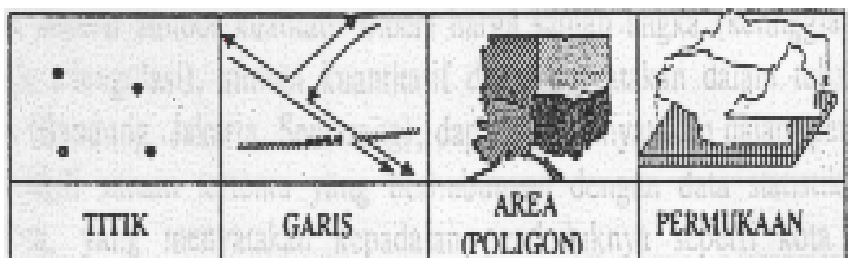
\includegraphics[width=1\textwidth]{figures/dataspasial.JPEG}}
	\caption{data spasial berikut berupa titik, garis, poligon (2-D), permukaan (3-D).}
	\label{dataspasial}
	\end{figure}

Dan arti dari gambar diatas adalah :
Format Titik 						
- Memiliki koordinat tunggal 		
- Tanpa memiliki panjang 			
- Tanpa memiliki luasan

Format Garis
- memiliki koordinat titik awal dan akhir		
- memiliki panjang tanpa luasan

Format Poligon 					
- memiliki koordinat titik awal dan akhir
-memiliki panjang dan luasan 		

Format Permukaan
- memiliki area koordinat vertikal
- memiliki area dengan ketinggian

\item Information
Informasi berasal dari kata pengolahan sejumlah data. Di dalam GIS informasi mempunyai
volume terbesar. Dan setiap object geografi memiliki setting datanya tersendiri karena 
tidak sepenuhnya data yang ada dapat terwakili didalam peta. Maka, semua data harus
diasosiasikan pada objek spasial yang mampu membuat peta menjadi intelligent.

\item System
Pengertian dari suatu sistem merupakan kumpulan elemen-elemen yang saling berintegrasi 
dan berinterdependensi dalam sebuah lingkungan yang dinamis untuk mencapai tujuan tertentu.
\end{enumerate}

\subsection{Definisi GIS (Geography Information and System)}
Dan defenisi dari GIS dapat selalu berubah karena GIS adalah bidang kajian ilmu 
dan teknologi yang masih baru. Beberapa defenisi dari Geographical Information System yaitu:
\begin{enumerate}
\item Definisi GIS menurut(Rhind, 1988):
yaitu : GIS is a computer system for collecting, checking, integrating and analyzing
information related to the surface of the earth.

\item Definisi GIS menurut(Marble \& Peuquet, 1983) and (Parker,
1988; Ozemoy et al., 1981; Burrough, 1986):
yaitu : GIS deals with space-time data and often but not necessarily, employs computer
hardware and software.

\item Difinisi GIS menurut (Purwadhi, 1994):
- SIG adalah suatu sistem yang mampu mengorganisir perangkat keras (hardware),
perangkat lunak (software), dan data, serta dapat mendaya dan digunakan sistem
penyimpanan, pengolahan, maupun analisis data yang dilakukan secara simultan, sehingga dapat
diperoleh seluruh informasi yang berkaitan secara langsung dengan aspek keruangan.
- SIG adalah manajemen data spasial dan data non-spasial yang berbasis komputer
dengan menggunakan tiga karakteristik dasar, yaitu: 
(i) memiliki fenomena yang aktual (variabel data non-lokasi) dan berhubungan 
dengan topik permasalahan di lokasi bersangkutan; 
(ii) merupakan suatu kejadian di suatu lokasi tertentu; 
(iii) memiliki dimensi waktu. Alasan GIS dibutuhkan adalah karena untuk data spasial 
penanganannya sangat sulit karena peta dan data statistik cepat mengalami kadaluarsa 
sehingga tidak ada pelayanan penyediaan data dan informasi yang diberikan menjadi tidak akurat.
\end{enumerate} 

Berikut merupakan keistimewaan analisa dengan Geographical Information System (GIS) yaitu:
\begin{enumerate}
\item Analisa Proximity
Analisa Proximity adalah geografi yang berbasis pada jarak antar layer.
Didalam analisis proximity GIS menggunakan proses yang disebut dengan buffering
yaitu membangun lapisan pendukung sekitar layer dalam jarak tertentu agar dapat menentukan
dekatnya hugungan antara sifat bagian yang ada.
\item Analisa Overlay
Analisa Overlay adalah proses integrasi data dari lapisan-lapisan layer yang berbeda (overlay).
Yang secara analisa membutuhkan lebih dari satu layer yang akan ditumpang susun secara
fisik agar dapat dianalisa secara visual.
\end{enumerate}

Maka artikel :
	Dalam sebuah artikel dari husein yang menyebutkan bahwa  GIS merupakan pemahaman dari
	Geography, Information dan System \cite{husein2006konsep}.

\section{Geographic Information System (GIS): Introduction to the computer perspective}
Sistem Informasi Geografi (GIS) diartikan sebagai sistem untuk menyimpan, memeriksa, 
mengintegrasi, memanipulasi, menganalisis dan memaparkan data yang berkaitan dengan semua 
ruang yang berhubungan dengan keadaan bumi.
Maka artikel :
	Dalam sebuah artikel dari prahasta yang menyebutkan bahwa  GIS merupakan menyimpan, memeriksa, mengintegrasi, memanipulasi, menganalisis dan memaparkan data yang berkaitan dengan semua ruang yang berhubungan dengan keadaan bumi., Information dan System \cite{prahasta2009sistem}.

\subsection{Pengenalan GIS atau Geography Information System}
1. GIS atau dikenal dengan Sistem Informasi Geografi ditunjukan sebagai sistem yang mampu menyimpan, memeriksa, mengintegrasikan, memanipulasi, menganalisis dan memaparkan data-data yang terkait dengan spasial yang merunjuk terhadap bagian bumi. (Jabatan Alam Sekitar, 1987).

2. GIS merupakan satu set lat untuk mengumpulkan, menyimpan, mendapatkan, mengubah dan memaparkan data ruang dari keadaan  bumi yang sebenarnya untuk keperluan tertentu (Burrough, 1986).

3. GIS adalah setiap set manual atau prosedur komputer yang digunakan untuk menyimpan dan memanipulasi data geografis yang tersedia (Arronoff, 1989).

4. GIS merangkum keadaan bumi dengan peranti atau perangkat tertentu yang digunakan untuk peta input atau peta produk, bersama-sama dengan dengan sistem komunikasi yang diperlukan untuk dijadikan sebagai penghubung berbagai unsur. (Star \& Ester, 1990).

5. GIS adalah suatu sistem untuk membantu dalam membangunkan model tertentu yang mustahil untuk dijadikan sintesi data yang banyak. (Martin, 1996).

\subsection{Komponen GIS atau Geography Information System}
Komponen GIS sendiri dibagikan menjadi 3 komponen, yaitu :
Sistem Komputer (perkakas dan sistem operasi), Software GIS
(ArcGIS), database GIS, methode GIS (Prosedur analisis), People (Orang-orang yang menggunakan GIS/User).
Pada gambar \ref{komponenGIS} dijelaskan bahwa kompnen GIS sebagai berikut.

\begin{figure}[ht]
	\centerline{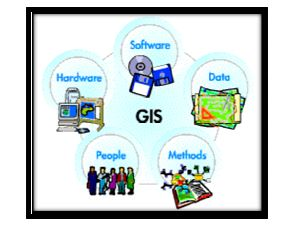
\includegraphics[width=1\textwidth]{figures/komponenGIS.JPG}}
	\caption{komponen GIS.}
	\label{komponenGIS}
	\end{figure}

\subsubsection{Komponen GIS atau Geography Information System}
sesuai dengan gambar diatas komponen GIS dibagi menjadi 3 bagian, yaitu :
1. Sistem Komputer (perkakas dan sistem operasi), merupakan hardware dari sebuah sistem GIS. Perkakas terdiri dari monitor, unit sistem atau CPU, keyboard dan mouse (Heywood et al., 2002). Teknologi komputer harus memiliki kemampuan kuasa
yang tinggi untuk menjalankan perisian GIS.

2. Software GIS , merupakan ArcGIS untuk tujuan perancangan, pengurusan ataupun pemodelan pada kebutuhan tertentu.

3. Database GIS , merupakan tempat yang melibatkan data GIS baik data spatial dan pengurusan datanya. memori untuk menyimpan jumlah data yang besar dan mempunyai kualitas yang baik dengan resolusi tinggi pada skrin grafik warna (untuk membantu dalam menentukan maklumat yang dihasilkan atau diberikan melalui penggunaan warna yang berbeda).

4. Methode GIS , merupakan prosedur dari analisis sistem GIS. yang melibatkan proses input, proses menyimpan, proses mengurus, proses menukar, proses menganalisis, dan proses output yang hanya melibatkan perisian GIS untuk mengatur sistem dan data-data tersebut (Heywood et al., 2002 )

5. People , merupakan orang-orang yang menggunakan sistem GIS. atau orang yang mengendaliakn proses input-output sistem GIS. 

\subsection{Kaedah GIS atau Geography Information System}
Berdasarkan pemahaman diatas, kaedah GIS juga merupakan salah satu komponen penting untuk mengatur sistem GIS sesuai dengan penjelasan sebelumnya. Kaedah-kaedah ini terdiri dari input
data spatial, pengurusan data atribut, paparan data, penerokaan data, analisis dan pemodelan data GIS;
yang dijelaskan oleh gambar sebagai berikut:
Pada gambar \ref{kaedahGIS} dijelaskan bahwa kaedah GIS sebagai berikut.
\begin{figure}[ht]
	\centerline{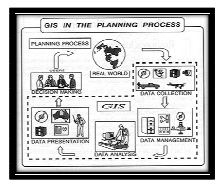
\includegraphics[width=1\textwidth]{figures/kaedahGIS.JPG}}
	\caption{kaedah GIS.}
	\label{kaedahGIS}
	\end{figure}

\subsubsection{Kaedah GIS atau Geography Information System}
1. Input data spatial
Merupakan langkah awal agar terciptanya data baru, dengan cara menginputkan data dan sistem GIS akan menyuntingnya dalam bentuk transformasi geometri yang nantinya akan menghasilkannya kedalam bentuk hard copy. (Chang, 2008) 
(Heywood et al., 2002).

2. Pengurusan data artibut
Merupakan langkah selanjutnya agar sumber peta dapat dipindahkan kepada peta digital yang dapat dibaca oleh GIS.
(Chang, 2008) (Worboy \& Duckham, 2003) (Heywood et al., 2002)

3. Pengumpulan data
Merupakan aktivitas untuk proses melakukan eksplorasi lebih jauh dalam meneliti ciri kesamaa dalam suatu graf peta yang berbeda. (Worboy \& Duckham, 2003).

4. Analisis data
Merupakan cara untuk memaparkan dan memanipulasi data yang didapat. Dengan menggunakan 2 jenis format, yaitu :
- data vektor : melibatkan beberapa kaedah seperti penimbalan / buffering, penindihan/overlay, pengukuran jarak, statik ruang, dan manipulasi peta.
- data raster : menaganalisis pengumpulan data tempatan, kaedah kejiranan, kaedah berzon, dan kaedah operasi global.
(Chang, 2008) (Worboy \& Duckham, 2003) (Heywood et al., 2002)

5. Paparan data dan output data
Dasarnya disediakan untuk tujuan pemaparan hasil dari analisis data yang fungsinya ditujukan untuk pengguna.

6. Aplikasi GIS
Digunakan untuk keperluan tertentu dan bersifat umum bagi masyarakat tergantung keperluan penggunanya. 
(Heywood et al., 2002).

Pada gambar \ref{aplikasiGIS} dijelaskan bahwa aplikasi GIS sesuai keperluan penggunan sebagai berikut.
\begin{figure}[ht]
	\centerline{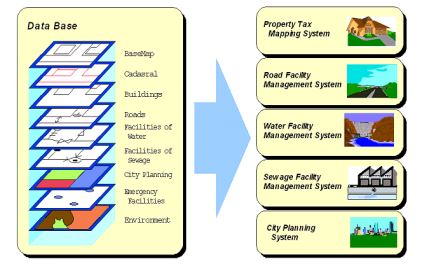
\includegraphics[width=1\textwidth]{figures/aplikasiGIS.JPG}}
	\caption{aplikasi GIS.}
	\label{aplikasiGIS}
	\end{figure}
Maka artikel :
	Dalam sebuah artikel dari hua yang menyebutkan bahwa  GIS memiliki kaedah dan komponen, Information dan System \cite{hua2017sistem}.

\subsection{Kesimpulan GIS atau Geography Information System}
Kesimpulannya, GIS merupakan alat yang penting dalam perspektif komputer pada masa kini dikarenakan GIS
mempunyai kemampuan aplikasi dalam berbagai bidang, misalnya dalam proses perancangan bandar dan kartografi,
penilaian kesan alam sekitar dan pengurusan sumber asli. GIS juga memainkan peranan dalam perspektif perniagaan,
dimana alat ini sangat bermanfaat dalam pengiklanan dan pemasaran, jualan, dan logistik 
mampu digunakan untuk mencari dan meningkatkan perniagaan seperti tapak perniagaan yang strategik. Sebagai umum, pengguna GIS dapat dilibatkan dengan agensi-agensi penguatkuasaan undang-undang, strategi
perancangan, perhutanan, industri, pemberdayaan alam, perencanaan kota, profesional
telekomunikasi, kesehatan, pengangkutan, geografi, dan pembangunan pemasaran. 
Penjelasan ini menyediakan platform untuk memahami lebih lanjut tentang komponen, kaedah, dan aplikasi GIS, 
untuk mempelajari tentang alat GIS.
\subsection{Saran GIS atau Geography Information System}
GIS dapat diaplikasikan di dalam kehidupan sehari-hari untuk memenuhi kebutuhan dan dapat membantu kebutuhan setiap masyarakat menjadi lebih baik dan lebih bermanfaat. Karena dengan memanfaatkan kemajuan teknologi maka teknologi yang digunakan akan ikut turut serta terus perkembang untuk menyesuaikan pemenuhan kebutuhan setiap pengguna yaitu masyarakat. Demikian kesimpulan dan saran yang dapat disampaikan kurang lebihnya mohon maaf dan terimakasih.

\subsection{SIG mempresentasikan real world dengan data spasial yang terbagi atas 2 model data, yaitu:}
1. Vektor, Bumi dalam data vector direpresentasikan sebagai mozaik yang terdiri atas garis, polygon, titik,
dan noders.
Model data vector merupakan model data yang paling banyak digunakan, model ini berbasiskan
pada titik dengan koordinat (x,y) untuk membangun objek spasialnya. Objek yang dibangun
dibagi menjadi tiga bagian, yaitu: titik, garis, dan area (polygon).
Keuntungan dari data vector, yaitu: ketepatan dalam merepresentasikan fitur titik, batasan dan
garis lurus.
2. Raster, Data raster adalah data yang dihasilkan dari sistem pengindraan yang jauh. Pada data raster,
objek geografis direpresentasikan sebagai struktur sel grid yang disebut pixel. Resolusi pada data
raster tergantung pada ukuran pixel-nya.
Maka, resolusi pixel menggambarkan ukuran sebenarnya dari permukaan bumi yang diwakili
oleh setiap pixel pada citra. Semakin tinggi resolusinya, semakin kecil permukaan bumi yang
direpresentasikan oleh suatu sel. Data raster cocok untuk merepresentasikan batas-batas yang
berubah secara gradual, seperti jenis tanah, vegetasi, suhu tanah, dan kelembaban tanah.


\chapter[Sejarah Bumi]
{Pengantar\\ Sejarah Bumi}
% Nama Kelompok : Kelompok 4
% Akbar Pambudi Utomo (1154094) 
% Andi Nurfadilah Ali (1154041)
% Andi Wadi Afryandika (1154113)
% Hanna Theresia Siregar (1154009)
% Julham Ramadhana (1154069)
% Pebridayanti Hasibuan (1154118)

\section{Sejarah Bumi}
Bumi merupakan planet atau rumah kita dalam kedudukan di tata surya. peradaban kuno percaya bahwa bumi itu datar, dengan langit berputar-putar sekali sehari. secara umum yang diyakini bahwa kehidupan di Bumi dimulai di Bumi itu sendiri, beberapa waktu setelah terbentuknya planet antara 4000-5000 juta tahun yang lalu. namun ada yang berpendapat bahwa kehidupan diluar bumi itu ada, tetap kita tidak memiliki bukti pasti tentang kehidupan di tempat lain. yang perlu kita ketahui bumi berada pada galaksi bimasakti dimana terdapat matahari sebagai sistem bintang.
Dalam Geologi sendiri atau biasa disebut sebagai ilmu pengetahuan tentang Kebumian yang mempelajari segala sesuatu mengenai planet Bumi beserta isinya yang pernah ada. Dalam Geologi juga akan dibahas tentang sifat-sifat dan bahan- bahan yang membentuk bumi itu apa, serta struktur dan proses-proses yang bekerja baik didalam maupun dibagian teratas permukaan bumi, kedudukannya di Alam Semesta hingga sekarang. Geologi merupakan ilmu pengetahuan yang komplek, mempunyai pembahasan materi yang beraneka ragam namun juga merupakan ilmu pengetahuan yang enak dipelajari. Sebagai landasan prinsip untuk dapat mempelajari ilmu geologi adalah bahwasanya kita harus menganggap bumi ini sebagai suatu benda yang secara dinamis berubah sepanjang masa, setiap saat dan setiap detik. 
Pemikiran geologi modern dikenalkan oleh Huttonian revolution mengemukakan pemikiran-pemikirannya sebagai berikut:
1. Bahwasanya proeses-proses alam yang sekarang ini menyebabkan perubahan pada permukaan bumi, juga bekerja sepanjang umur dari bumi ini. 
2. Ia juga mengamati bahwa proses-proses tersebut yang walaupun bekerja sangat lambat, tetapi pada akhirnya mampu menyebabkan terjadinya perubahan-perubahan yang sangat besar pada bumi. 
3. Bahwa bumi ini sangat dinamis, yang berarti mengalami perubahan-perubahan yang terus-menerus mengikuti suatu pola daur (siklus) yang berulang-ulang.
Bumi sendiri berada di kawasan dimana terjadinya tumpang tindih antara litosfer (daratan) bagian padat dari bumi, hidrosfer (perairan), dan atmosfer (udara) yang menyelubungi bumi dengan zarah-zarah dan benda-benda yang mengisinya.
Dalam sejarah terbentuknya bumi sewaktu SMA kita pernah mempelajari teori-teori terbentuknya bumi dalam pelajaran geografi.\cite{wetherill1990formation}

\subsection{Teori-teori terbentuknya Bumi}
\subsubsection{1.Teori Kabut Kant-Laplace}
\begin{figure} [ht]
	\centerline{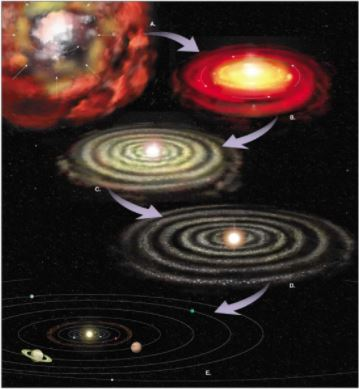
\includegraphics[width=1\textwidth]{figures/teorikabutnebula.JPG}}
	\caption{Gambar Teori Nebula}
	\label{teorikabutnebula}
	\end{figure}
	Pada Gambar berikut \ref{teorikabutnebula} adalah gambar dari Teori Kabut Nebula.
Teori ini dikenal dengan teori kabut (nebula) yang dikemukakan oleh Immanuel Kant (1755) dan Pierre de Laplace (1796). dalam teori ini dikemukakan bahwa di jagat raya terdapat gas yang kemudian berkumpul menjadi kabut(nebula). gaya tarik-menarik antargas ini membentuk kumpulan kabut yang sangat besar dan berputas semakin cepat sehingga materi kabut bagian khatulistiwa terlempar memisah dan memadat(karena pendinginan), bagian yang terlempar inilah yang kemudian menjadi sebuah planet dalam tatasurya. Bumi baru terus bertumbuh sampai suhu interiornya cukup panas untuk melelehkan logam siderofil. Dengan massa jenis yang lebih tinggi dari silikat, akhirnya logam ini tenggelam. Proses ini terjadi 10 juta tahun setelah Bumi mulai terbentuk, dan menghasilkan struktur Bumi yang berlapis-lapis dan mengakibatkan terbentuknya medan magnet. J. A. Jacobs merupakan orang pertama yang menunjukkan bahwa inti dalam—bagian dalam yang padat berbeda dari inti luar yang padat—membeku dan mengembang keluar inti luar yang cair dikarenakan bagian dalam bumi yang makin mendingin (sekitar 100° C per miliar tahun. Ekstrapolasi dari pengamatan ini memperkirakan bahwa inti terbentuk pada masa 2–4 miliar tahun yang lalu. Jika ini benar maka berarti bahwa inti bumi bukanlah fitur primordial yang berasal selama pembentukan planet.

\subsubsection{2.Teori Planetesimal}
\begin{figure} [ht]
	\centerline{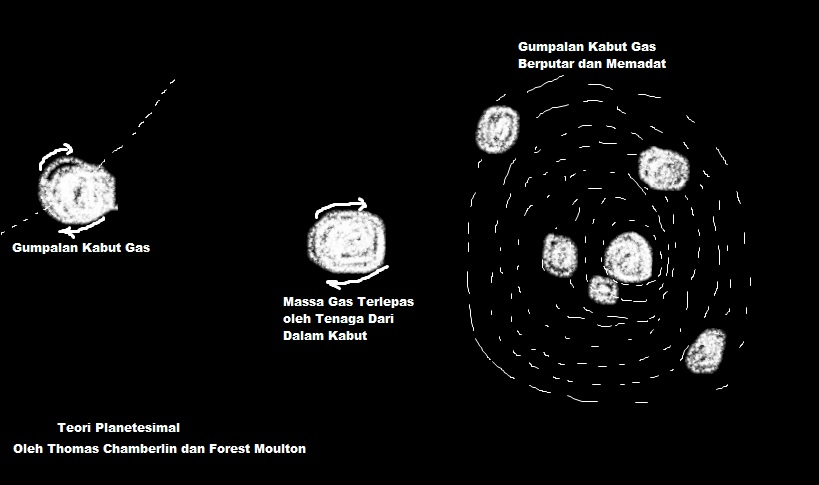
\includegraphics[width=1\textwidth]{figures/teoriplanetesimal.JPG}}
	\caption{Gambar Teori Planetesimal}
	\label{teoriplanetesimal}
	\end{figure}
	Pada Gambar berikut \ref{teoriplanetesimal} adalah gambar dari Teori Planetesimal.
seabad kemudian sesudah teori kabut tersebut muncul teori Planetesimal yang dikemukakan oleh Chamberlin dan Moulton. Teori ini mengungkapkan bahwa pada mulanya telah terdapat Matahari asal. pada suatu ketika, matahari asal ini didedakti sebuah bintang besar yang menyebabkan terjadinya penarikan pada bagian matahari. Akibat tenaga tarik menarik tadi, terjadilah ledakan yang dasyat. Gas yang meledak ini keluar dari atmosfer matahari, kemudian mengembun dan membeku sebagai benda-benda yang padat(disebut planetesimal). Planetesimal ini dalam perkembangannya menjadi planet-planet, dan salah satunya planet bumi kita.

\subsubsection{3.Teori Pasang Surut Gas}
\begin{figure} [ht]
	\centerline{\includegraphics[width=1\textwidth]{figures/teoripasangsurut.JPG}}
	\caption{Gambar Pasang Surut}
	\label{teoripasangsurut}
	\end{figure}
	Pada Gambar berikut \ref{teoripasangsurut} adalah gambar dari Teori Pasang Surut.
Teori ini dikemukakan oleh Jeans dan Jeffreys, yakni bahwa sebuah bintang besar mendekati matahari dalam jarak pendek, sehingga menyebabkan terjadinya pasang surut pada tubuh matahari. dalam lidah yang panas ini terjadi perapatan gas-gas dan akhirnya kolom-kolom ini akan pecah, lalu berpisah menjadi benda-benda tersendiri yaitu planet-planet. bintang besar yang menyebabkan penarikan pad abagian-bagian tubuh matahari tadi melanjutkan perjalanan di jagat raya, sehingga lambat laun akan hilang pengaruhnya terhadapt planet-planet yang terbentuk tadi, lalu planet-planet itu akan mengelilingi matahari dan mengalami proses pendinginan, proses pendinginan berjalan lambat pada planet besar seperti yupiter dan saturnus, sedangkan planet kecil seperti bumi mengalami proses pendinginan yang relatif lebih cepat.

\subsubsection{4. Teori Bintang Kembar}
\begin{figure} [ht]
	\centerline{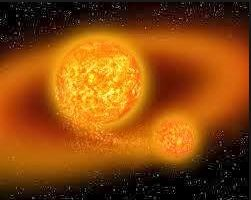
\includegraphics[width=1\textwidth]{figures/teoribintangkembar.JPG}}
	\caption{Gambar Teori Bintang Kembar}
	\label{teoribintangkembar}
	\end{figure}
	Pada Gambar berikut \ref{teoribintangkembar} adalah gambar dari Teori Bintang Kembar.
Teori ini dikemukakan oleh seorang ahli astronomi R. A. Lyttleton. Menurut teori ini, galaksi berasal dari kombinasi bintang kembar. Salah satu bintang meledak sehingga banyak materi yang terlempar. Karena bintang yang tidak meledak mempunyai gaya gravitasi yang masih kuat, maka sebaran pecahan ledakan bintang tersebut mengelilingi bintang yang tidak meledak. Bintang yang tidak meledak itu adalah matahari, sedangkan pecahan bintang yang lain itu adalah planet-planet yang mengelilinginya.

\subsubsection{5. Teori Dentuman Besar (Big Bang Teory)}
\begin{figure} [ht]
	\centerline{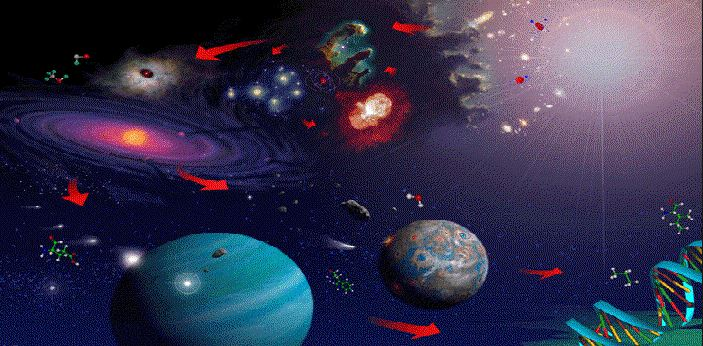
\includegraphics[width=1\textwidth]{figures/teoribigbang.JPG}}
	\caption{teoribigbang}
	\label{teoribigbang}
	\end{figure}
	Pada Gambar berikut \ref{teoribigbang} adalah gambar dari Teori Dentuman Besar(BigBang).
Pada Teori ini berdasarkan dari asumsi adanya massa yang sangat besar dan mempunyai massa jenis sangat besar. Adanya reaksi inti menyebabkan massa tersebut meledak hebat. Massa tersebut kemudian mengembang dengan sifat sangat cepat menjauhi pusat ledakan, karena danya gravitasi, maka bintang yang paling kuat gravitasinya akan menjadi pusatnya.
Dari berbagai teori, teori ini yang paling banyak didukung oleh para ilmuwan.

\section{Pendapat Tentang Sejarah Bumi}
Bumi terbentuk sekitar 4,54 miliar (4,54×109) tahun yang lalu melalui akresi dari nebula matahari. Pelepasan gas vulkanik diduga menciptakan atmosfer tua yang nyaris tidak beroksigen dan beracun bagi manusia dan sebagian besar makhluk hidup masa kini. Sebagian besar permukaan Bumi meleleh karena vulkanisme ekstrem dan sering bertabrakan dengan benda angkasa lain. Sebuah tabrakan besar diduga menyebabkan kemiringan sumbu Bumi dan menghasilkan Bulan. Seiring waktu, Bumi mendingin dan membentuk kerak padat dan memungkinkan cairan tercipta di permukaannya. Bentuk kehidupan pertama muncul antara 2,8 dan 2,5 miliar tahun yang lalu. Kehidupan fotosintesis muncul sekitar 2 miliar tahun yang lalu, nan memperkaya oksigen di atmosfer. Sebagian besar makhluk hidup masih berukuran kecil dan mikroskopis, sampai akhirnya makhluk hidup multiseluler kompleks mulai lahir sekitar 580 juta tahun yang lalu. Pada periode Kambrium, Bumi mengalami diversifikasi filum besar-besaran yang sangat cepat. Perubahan biologis dan geologis terus terjadi di planet ini sejak terbentuk. Organisme terus berevolusi, berubah menjadi bentuk baru atau punah seiring perubahan Bumi. Proses tektonik lempeng memainkan peran penting dalam pembentukan lautan dan benua di Bumi, termasuk kehidupan di dalamnya. Biosfer memiliki dampak besar terhadap atmosfer dan kondisi abiotik lainnya di planet ini, seperti pembentukan lapisan ozon, proliferasi oksigen, dan penciptaan tanah.Dalam sebuah artikel dari zuhdi2012sistem yang menyebutkan bahwa Bumi merupakan salah satu planet yang berada dalam tata surya yang diduga terbentuk dari pecahan-pecahan bintan pada jutaan tahun yang lalu, dan kemudian terperangkapa pada gravitasi matahari sehinggan akan selalu mengelilingi matahari. Menurut Hukum Newton kenapa planet dapat bertahan dalam pergerakan keliling atau biasa disebut revolusi dikarenakan planet melakukan gerak melingkar yang menimbulkan gaya sentifugal yang besarnya  dengan gaya gravitasi namun berlawanan arah. Gaya gravitasi ini sendiri akan berkurang sesuai dengan semakin jauhnya jarak planet dari matahari, sedangkan gaya sentrifugal  akan tergantung pada kecepatan gerak melingkar planet. Semakin cepat gerakan tersebut maka akan semakin besar daya sentifugal. Bila secara kebetulan kedua gaya ini memiliki kecepatan yang sama besar, maka planet akan terjebak mengelilingi matahari. Pada saat tata surya terbentuk diperkirakan terdapat jutaan planet. Akan tetapi sebagian terjatuh ke matahari atau terlempar lepas dari pengaruh matahari. Selain berkeliling, planet juga akan bergerak memutari pororsnya (rotasi). Gerak rotasi ini sendiri berlangsung dalan waktu lama sehingga membuat planet berbentuk seperti bola. Pada masa lalu, planet planet bukanlah sebuah benda padat, melainkan berupa magma atau berupa cairan batu. Bagian padat pada planet terbentuk selama proses pendinginan dan terjadi pada bagian kulit terluar dari planet tersebut. Bentuk Bumi sendiri yang dikatakan berbentuk bola tidakalah sempurna. Gerak Rotasi telah mengubah bentuk bumi menjadi agak cepat terhadap kedua kutubnya.\cite{zuhdi2012sistem}


Sejarah pembentukan Bumi yang dipelajari dalam materi pelajaran Geografi cenderung memiliki sifat abstrak yang akan lebih mudah dimengerti, jika memakai media yang cocok. Salah satu Inovasi pembelajaran yang tepat untuk dilakukan adalah menggunakan kartu indeks dan media film. Media seperti kartu indeks yang dipergunakan sebaga salah satu upaya yang memudahkan peserta didik agar mengingat konsep-konsep materi yang sedang dipelajari sedangkan media film sendiri merupakan media visual yang akan menjelaskan dengan lebih konkrit tentang fenomena bumi. Dalam sebuah artikel dari @article{widiyati2011meningkatkan menyebutkan bahwa Pmebentukan Bumi dengan kategori Continental Drift Theory atau biasa disebut dengan teori pengapungan benua yang dikemukan oleh Alfred Wegener pada tahun 1912 mengemukakan bahwa sampai sekitar 255 juta tahun lalu, di bumi baru ada satu benua dan samudera yang sangat luas. Benua raksasa ini sendiri dinamakan pangea, sedangkan kawasan samudera yang mengapitnya itu mengalami retakan-retakan dan pecah. Sekitar 135 juta tahun lalu, benua raksasa tersebut pecah menjadi dua, yaitu pecahan benua di sebelah utara yang dinamakan Lauransia dan dibagian selatan dinamakan gondwana.
\cite{widiyati2011meningkatkan}



\chapter[Kordinat Indonesia]
{Pengantar\\ Kordinat Indonesia}
% Nama kelompok : 3
% Kelas : D4 Teknik Informatika 3C
% 1. Kezia Tirza Naramessakh (1154093)
% 2. Mariani Rospilinda Siki (1154107)
% 3. Doli Jonviter Nt Simbolon (1154016)
% 4. Benedictus Simantupang (1154116)
% 5. Dimas Mathovani 


\section{Koordinat Lintang Utara, Lintang Selatan, Bujur Timur, Bujur Barat}
Koordinat digunakan untuk menunjukkan suatu titik di Bumi berdasarkan garis lintang dan garis bujur. Koordinat dibagi menjadi dua bagian irisan yaitu irisan melintang yang disebut dengan garis lintang mulai dari khatulistiwa, membesar ke arah kutub(utara maupun selatan) sedangkan yang lain membuju r mulai dari garis Greenwhich membesar ke arah barat dan timur. Satuan skala koordinat dibagi dalam derajat lintang 0* sampai 90* dan bujur 0* sampai 180*. Koordinat ini ditulis dalam satuan derajat, menit, dan detik, misalnya 110*35'32", dan seterusnya. Untuk membagi dunia dalam wilayah utara dan selatan, maka ditentukan sebuah garis yang tepat berada di tengah, yaitu garis Equator / Khatulistiwa. Untuk membagi wilayah timur dan barat, maka ditentukan sebuah garis Prime meridian yang terletak di kota Greenwich (Inggris), dan perpotongannya bertemu di wilayah laut pasific, yakni memotong kepulauan Fiji.
Koordinat pada gambar \ref{Koordinat} di jelaskan garis Lintang dan Bujur
\begin{figure}[ht]
	\centerline{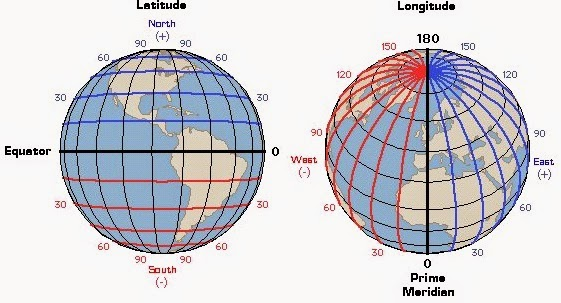
\includegraphics[width=1\textwidth]{figures/Koordinat.JPG}}
	\caption{Koordinat Lintang dan Bujur}
	\label{Koordinat}
	\end{figure}

\subsection{Sistem Koordinat}
Dalam artikel Zuhdi menjelaskan Koordinat dimaksudkan untuk memberikan pengalamatan terhadap setiap lokasi di permukaan bumi. Pengalamatan dengan sistem koordinat didasarkan atas jarak timur-barat dan utara-selatan suatu tempat dari suatu titik pangkal tertentu. Jarak diukur dalam satuan derajat sudut yang dibentuk dari titik pangkal ke posisi tersebut melalui pusat bumi. Sedangkan titik pangkal ditetapkan berada di perpotongan belahan utara-selatan bumi (garis khatulistiwa) dengan garis yang membelah bumi timur-barat melalui kota GreenWhich di Inggris. 
Untuk lebih jelas tentang bentuk titik koordinat lihat pada gambar \ref{sistemkoordinat} dibawah ini :
\begin{figure}[ht]
	\centerline{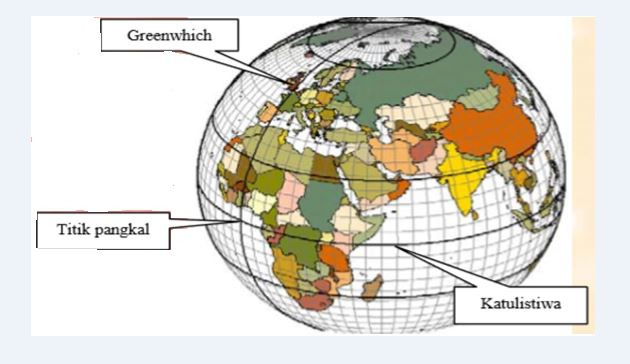
\includegraphics[width=1\textwidth]{figures/sistemkoordinat.JPG}}
	\caption{Bentuk titik Koordinat}
	\label{sistemkoordinat}
	\end{figure}

Baik garis lintang maupun garis bujur diukur dalam derjat dan dibagi lagi dalam menit dan detik. 1 derajat garis bujur diukur lapangan sama dengan 11,32 km. Satuan derajat bisa juga disebut jam sehingga setiap derajat terbagi menjaid 60 menit dan setiap menit terbagi menjadi 60 detik. Dalam penulisan letak astronomis contohnya 60 derajat 23' 15"S, maka dibaca sebagai 60 derajat 23 menit 15 detik lintang selatan. pada sistem pemetaan internasional huruf U sebagai lintang utara diganti dengan huruf N (north). Besar sudut dalam sistem koordinat geografik dapat dinyatakan dalam dua cara, yaitu dengan satuan DMS(Degree Minute Second) atau satuan DD(Decimal Degree), dalam sistem satuan DMS, setiap derajat sudut dibagi menjadi 60 menit dan setiap menitnya dibagi lagi menjadi 60 detik. Penulisannya dinyatakan sebagai dd°mm'ss". Sedangkan pada sistem satuan setiap derajatnya dinyatakan dalam pecahan decimal (pecahan berkoma). Baik dalam DMS maupun DD, perlu diketahui berapa ketelitian suatu nilai koordinat. Karena di wilayah khatulistiwa jarak 1° sama dengan jarak 111321 meter. Maka perlu diperhatikan keselahan yang terjaddi jika kita mengabaikan suatu angka menit atau detik pada DMS atau suatu nilai digit dalam koordinat DD. Pada sistem DD, perlu diperhatikan jarak yang diwakili oleh setiap digit dibelakang koma. Perubahan satu satuan padaa digitt pertamma dii belakang koma mempunyai nilai jarak lebih dari 11 Km. Perubahan satu unit pada digit keduat dibelakang koma berarti 1,1 Km. Demikian seterusnya. Berarti jika kita misalnya hanya mentolerir kesalahan sampai 100 m, maka koordinat DD harus dibuat setidaknya sampai 4 digit di belakang koma. Kombinasi antara garis lintang dan garis bujur akan membentuk sutau koordinat lokasi di permukaan bumi dengan sumbu x sebagai garis lintang dan sumbu y sebagai garis bujur dalam koordinat kartesius. Pada Bujur/Longitude (X) merupakan garis yang perpindahannya secara vertical dan pada Lintang/Lattitude (Y) merupakan garis yang mempunyai perpindahan secara horizontal. \cite{zuhdi2012sistem}.

Lihat pada gambar \ref{lintangbujur} dibawah ini :
\begin{figure}[ht]
	\centerline{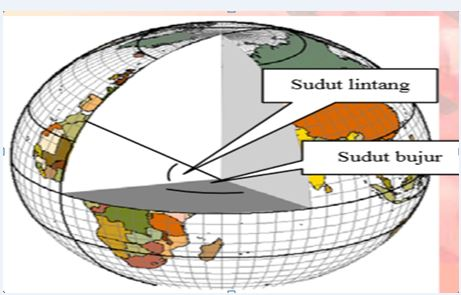
\includegraphics[width=1\textwidth]{figures/lintangbujur.JPG}}
	\caption{Titik Lintang dan Bujur}
	\label{lintangbujur}
	\end{figure}

\subsubsection{Garis Lintang}
Sebuah garis khayal yang digunakan untuk menentukan lokasi di Bumi terhadap garis khatulistiwa(utara atau selatan). Posisi lintang merupakan penghitungan sudut dari 0 derajat di khatulistiwa sampai ke +90 derajat di kutub utara dan -90 derajat di kutub selatan. Dalam bahasa indonesia lintang di sebelah utara khatulistiwa diberi nama Lintang Utara(LU), demikian pula lintang di sebelah selatan khatulistiwa diberi nama Lintang Selatan(LS). Lintang Utara dan Lintang Selatan menyatakan besarnya sudut antara posisi lintang dengan garis Khatulistiwa. Garis Khatulistiwa sendiri adalah lintang 0 derajat. 
Nilai koordinat lingtang dimulai dari garis lingkaran khatulistiwa yang diberi nilai 0 derajat. Selanjutnya garis lintang yang lain berupa lingkarang paralel (sejajar) katulistiwa berada disebelah utara dan selatan khatulistiwa. Lingkaran paralel di selatan disebut garis lintang selatan (LS) dan diberi nilai negatif, sedangkan lingkaran paralel diutara diberi nilai positif dan disebut garis lintang utara (LU). Nilai maksimum koordinat garis lintang adalah 90 derajat yaitu terletak di kutub-kutub bumi. 
Lingkaran paralel merupakan representasi garis lintang ini semakin mengecil ukurannya dengan semakin jauh dari katulistiwa. sehingga jarak 1 derajat timur-barat dari katulistiwa jauh lebih besar dari pada jarak 1 derajat timur-barat di tempat yang jauh dari katulistiwa. Di khtulistiwa 1 derajat timur-barat sama dengan 111.321 km, tapi di dekat kutub 1 derajat timur-barat hanya beberapa meter saja. itu sebabnya grid yang dibuat dari garis lintang dan garis bujur, tampak berupa sangkar dikatulistiwa dan berubah menjadi persegi didaerah kutub
lintang memiliki symbol phi dan menunjukkan sudut antara garis lurus dititik tertentu dengan bidang ekuator. Lintang ditentukan dalam angka derajat dimulai dari 0 derajat dan berakhir dengan 90 derajat. garis lintang ini membagi bumi menjadi belahan bumi utara dan selatan. garis ekuator atau khatulistiwa berada di lintang 0 derajat. Garis lintang biasa digunakan untuk melihat penyebaran iklim di bumi.
Latitude aau garis lintang adalah garis yang menentukan lokasi berada di sebelah utara atau selatan ekuator. garis lintang diukur mulai dari titik 0 derajat dari khatulistiwa sampai 90 derajat di kutub. Garis lintang digunakan untuk membatasi corak iklim di permukaan bumi, berikut ini merupakan pembagian iklim di bumi menurut batas garis lintang:
1. 23,5-23,5 LU/LS = iklim tropis
2. 23,5-40 LU/LS = iklim subtropis
3. 40 Lu-66,5 LU/LS = iklim sedang
4. 66,5-90 LU/LS = iklim kutub
Indonesia terletak antara 6 derajat Lintang Utara (LU) – 11 derajat Lintang Selatan (LS) dan diantara 95 derajat bujur timur – 141 derajat Bujur timur.
Adapun wilayah indonesia itu pada bagian paling utara yang ebrada di Pulau Weh di Nanggroe Aceh Darussalam yang terletak pada 6 derajat lintang utara, dan untuk daerah indonesia yang paling berada di selatan yaitu Pulau Roti di Nusa Tenggara Timur yang terletak pada 11 derajat lintang selatan. Kemudian mengacu pada letak lintangnya, di wilayah Indonesia berada pada 6 derajat lintang utara – 11 derajat lintang selatan, hal tersebut disebabkan indonesia mempunyai iklim tropis dengan beberapa ciri-ciri yaitu mempunyai hutan hujan tropis yang begitu luas dan mempunyai nilai ekonomis yang sangat tinggi, mendapatkan sinar matahari yang lama setiap sepanjang tahun, mempunyai curah hujan yang tinggi dan memiliki banyak penguapan sehingga akan meningkatkan kelembaban udara.
Pada gambar \ref{lintang} dijelaskan titik koordinat Lintang pada sumbuh Y :
\begin{figure}[ht]
	\centerline{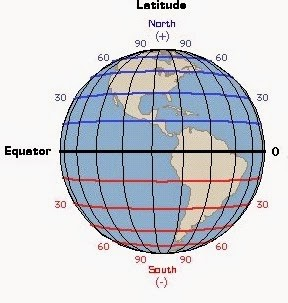
\includegraphics[width=1\textwidth]{figures/lintang.JPG}}
	\caption{Titik koordinat Lintang pada sumbuh Y}
	\label{lintang}
	\end{figure}

\subsubsection{Garis Bujur}
Menggambarkan lokasi sebuah tempat di timur atau barat Bumi dari sebuah garis utara-selatan yang disebut Meridian Utama. Longitude diberikan berdasarkan pengukuran sudut yang berkisar dari 0 derajat Meridian Utama ke +180 derajat arah timur dan -180 derajat arah barat. Tidak seperti lintang yang memiliki ekuator sebagai posisi awal alami, tidak ada posisi awal alami untuk bujur. Bujur di sebelah barat Meridian diberi nama Bujur Barat(BB), demikian pula bujur di sebelah timur Meridian diberi nama Bujur Timur(BT).
Nilai koordinat garis bujur dimulai dari bujur 0 derajat yaitu Greenwhich, kemudian memebersasr ke arah timur dan barat sampai bertemu kembali di garis batas tanggal internasional yaitu terletak di selat bering dnegan nilai 180 derajat. garis bujur 0 derajat disebut prime meridian atau meridian greenwhich. garsi bujur ke arah barat diberi nilai negatif dan disebut bujur barat (west longitude) serta disingkan BB. sedangkan garis bujur yang ke arah timur diberi nilai positif dan disebut bujur timur (east longitude) disingkat BT. nilai koordinatnya didasarkan atas besarnya sudut yang terbentuk dari bujur 0 ke garis bujur tersebut melalui pusat bumi.
Longitude atau garis bujur memiliki symbol lamda. garis bujur ini merupakan garis yang menunjukkan bagian barat dan timur dilihat dari titik pangkal yaitu di greenwich meridian. garis bujur emiliki batas maksimum yaiu 180 derajat ke arah timur dar GMT dan 180 derajat ke arah barat dari GMT. keduanya bertemu di garis internasional date line disekitar pasifik.
longitude atau garis bujur digunakan untuk menentukan lokasi diwilayah barat atau timur dari garis utara selatan yang sering disebut juga garis meridian. garis bujur digunakan untuk menentukan waktu dan tanggal.
Titik di barat bujur 0° dinamakan Bujur Barat sedangkan titik di timur 0° dinamakan Bujur Timur. Kombinasi garis lintang dan garis bujur ini berguna untuk menentukan suatu lokasi di permukaan bumi. Garis Lintang menandakan sumbu y dan garus bujur menandakan sumbu x dalam sistem koordinat cartesian. Sebagi contoh kota Sabang di pulau We berada pada koordinat 6oLU 95o BT, dan kota Merauke di Papua memiliki koordinat 11oLS dan 141oBT.
Indonesia berada pada 95 derajat bujur timur – 141 derajat bujur timur menyebabkan Indonesia mempunyai tiga waktu dan pada setiap waktu memiliki daerah tersendiri, sehingga Indonesia memiliki beberapa pembagian waktu yaitu Waktu Indonesia bagian timur atau WIT mencakup Papua, kepulauan Maluku dan pulau-pulau kecil disekitarnya. Untuk waktu indonesia bagian  timur mempunyai selisih waktu sebanyak 9 jam lebih awal dari Greenwich Mean time atau GMT. Kemudian untuk Waktu Indonesia bagian tengah atau WITA mencakup Nusa tenggara, kalimantan selatan, Pulau Sulawesi, Bali dan pulau-pulau kecil yang ada disekitarnya. Untuk Indonesia bagian tengah mempunyai selisih waktu sebanyak 8 jam yang lebih awal dari Greenwich mean time (GMT). Kemudian, untuk daerah waktu Indonesia bagian barat atau WIB yang mencakup Madura, Jawa, kalimantan barat, kalimantan tengah, Sumatera dan pulau-pulau kecil yang ada disekitarnya. Adapun waktu indonesia bagian barat mempunyai selisih waktu sebanyak 7 jam yang lebih awal dari Greenwich mean time.
Pada gambar \ref{bujur} dijelaskan titik koordinat Lintang pada sumbuh X :
\begin{figure}[ht]
	\centerline{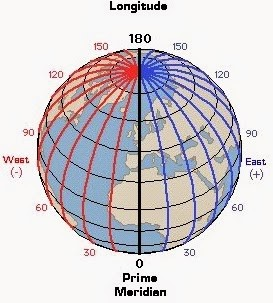
\includegraphics[width=1\textwidth]{figures/bujur.JPG}}
	\caption{Titik koordinat Bujur pada sumbuh X}
	\label{bujur}
	\end{figure}

\chapter[Kordinat Internasional]
{Pengantar\\ Kordinat Internasional}
% Nama Kelompok 2 : Latitude & Longitude
% Kelas : D4TI3C
% Adhika Dwi Cahya Putra (1154017)
% Haris Munandar Alwi (1154105)
% Muhammad Adam Nahdlotul Halimi (1154024)
% Tito Aryo Nugroho (1154074)
% Tomy Prawoto (1154121)

\section{latitude longitude}

\subsection{Latitude}
Latitude merupakan terjemahan bahasa inggris dari garis lintang. Garis lintang dapat disebut juga sebagai garis khatulistiwa (0 derajat), atau bisa disebut juga sebagai garis tengah bumi yang membagi antara belahan bumi bagian atas dan bumi bagian bawah.
Dalam sebuah buku karangan Maling \& Derek Hylton yang berjudul \"Coordinate System and Map Projections\" mengatakan bahwa garis lintang suatu titik dapat didefinisikan secara formal sebagai sudut yang diukur di tengah bumi di antara bidang equator dan jari jari yang ditarik ke titik. 
Pada garis lintang bagian utara bumi dilambangkan dengan tanda \verb|'+phi'| 
sedangkan garis lintang bagian selatan bumi dilambangkan dengan tanda \verb|'-phi'| 
\cite{maling2013coordinate}. 

	\begin{figure}[ht]
	\centerline{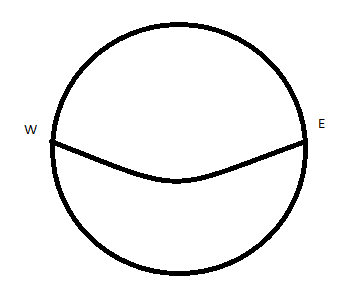
\includegraphics[width=1\textwidth]{figures/latitude.PNG}}
	\caption{Garis Lintang atau Latitude.}
	\label{latitude}
	\end{figure}
Pada gambar \ref{latitude} merupakan gambar latitude atau garis lintang yang membentang antara west(barat) sampai east(timur).
Garis lintang digunakan sebagai penanda dalam zona iklim di dunia. Dari +23 setengah derajat Lintang Utara sampai -23 setengah Lintang Selatan memiliki zona iklim tropis. Zona iklim tropis hanya memiliki dua musim, yaitu kemarau atau panas dan penghujan saja. Kemudian dari +23 setengah derajat Lintang utara sampai +66 setengah derajat Lintang utara memiliki zona iklim subtropis. Sama halnya bagian utara, bagian selatan yaitu -23 setengah derajat lintang selatan sampai -66 setengah derajat lintang selatan memiliki zona iklim subtropis. Daerah subtropis memiliki 4 musim, yaitu spring, summer, fall, dan winter. 

\subsection{Longitude}
Longitude merupakan terjemahan bahasa inggris dari garis bujur. Garis bujur biasa digunakan untuk menentukan waktu dan tanggal di dunia yang kita huni sekarang ini. Jika garis lintang atau latitude atau daerah khatulistiwa dianggap sebagai 0 derajat, maka garis bujur merupakan 0 derajat yang menghubungkan kutub utara dengan kutub selatan yang melawati kota Greenwich di Inggris. Garis bujur bagian barat kota Greenwich disebut sebagai Bujur Barat sedangkan garis bujur yang berada pada sebelah timur kota Greenwich disebut sebagai Bujur Timur. Inilah penyebab kenapa orang indonesia disebut sebagai orang timur.
	\begin{figure}[ht]
	\centerline{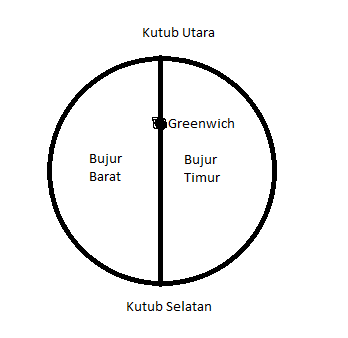
\includegraphics[width=1\textwidth]{figures/longitude.PNG}}
	\caption{Garis Bujur atau Longitude.}
	\label{longitude}
	\end{figure}
Pada gambar \ref{longitude} merupakan gambar longitude atau garis bujur yang menghubungkan kutub utara dengan kutub selatan. Garis ini melewati kota Greenwich di Inggris.
Garis bujur digunakan untuk pembagian zona waktu di dunia.

\section{LINTANG}

	Sudut lintang l
	Bayangkan Bumi adalah bola transparan (sebenarnya
	bentuknya agak oval; karena rotasi bumi, nya
	Khatulistiwa sedikit menonjol). Melalui Bumi yang transparan
	(gambar) kita bisa melihat bidang ekuatornya, dan bagian tengahnya
	titik adalah O, pusat bumi.
	Untuk menentukan garis lintang beberapa titik P di permukaan, tariklah
	radius OP ke titik itu. Maka sudut elevasi titik itu
	Di atas garis ekuator adalah garis lintang l - lintang utara jika utara
	dari garis khatulistiwa, lintang selatan (atau negatif) jika selatannya.
	Garis lintang. Di dunia bumi, garis lintang adalah lingkaran dengan ukuran yang berbeda. Itu
	terpanjang adalah khatulistiwa, yang garis lintangnya nol, sementara di kutub - di garis lintang
	90 ° utara dan 90 ° selatan (atau -90 °) lingkaran menyusut ke titik tertentu.

\section{GARIS BUJUR}
	Di dunia, garis bujur konstan ("meridian") meluas dari tiang ke kutub, seperti
	batas segmen pada jeruk kupas.
	Garis bujur atau "garis meridian"
	Setiap meridian harus melewati garis khatulistiwa. Karena ekuator adalah lingkaran, kita bisa
	bagilah itu - seperti lingkaran - ke dalam 360 derajat, dan bujur f dari sebuah titik adalah
	maka nilai yang ditandai dari divisi mana meridiannya memenuhi khatulistiwa.
	Apa nilai itu tergantung tentu saja dari mana kita mulai menghitung - di mana
	nol bujur adalah Untuk alasan historis, garis meridian melewati Astronomi Kerajaan yang lama
	Observatorium di Greenwich, Inggris, adalah yang dipilih sebagai nol bujur. Bertempat di Jl
	Tepi timur London, ibu kota Inggris, observatorium sekarang menjadi museum umum dan a
	band kuningan yang membentang di halamannya menandai "garis meridian utama". Wisatawan sering mendapatkan
	difoto saat mereka mengangkangnya - satu kaki di belahan bumi bagian timur, yang lainnya masuk belahan barat.
	Garis bujur juga disebut meridian, berasal dari bahasa Latin, dari meri, a
	variasi "medius" yang menunjukkan "tengah", dan diem, yang berarti "hari". Kata itu
	pernah berarti "siang", dan waktu sehari sebelum siang hari dikenal sebagai "ante meridian",
	sementara waktu setelah itu adalah "posting meridian." Singkatan hari ini a.m. dan p.m. datang
	Dari istilah ini, dan Matahari pada siang hari dikatakan "melewati meridian". Semua poin di
	garis bujur yang sama mengalami siang hari (dan jam lainnya) pada saat bersamaan dan
	oleh karena itu dikatakan sama "garis meridian", yang menjadi "meridian" untuk
	pendek.

\section{Waktu Lokal (LT) dan Zona Waktu}
	Garis bujur diukur dari nol sampai 180 ° BT dan 180 ° BB (atau -180 °), dan kedua 180-
	Gelombang longitudinal berbagi jalur yang sama, di tengah Samudera Pasifik.
	Saat Bumi berputar mengelilingi porosnya, kapanpun satu garis bujur - "siang hari
	meridian "- menghadap Matahari, dan pada saat itu, akan ada siang hari di mana-mana di atasnya
	jam Bumi telah mengalami rotasi penuh sehubungan dengan Matahari, dan meridian yang sama
	lagi wajah siang hari Jadi setiap jam Bumi berputar 360/24 = 15 derajat.
	Bila di lokasi Anda waktu 12 siang, 15 ° ke timur waktu adalah 1 p.m., karena itu adalah
	meridian yang dihadapi Matahari sejam yang lalu. Di sisi lain, 15 ° ke barat waktu adalah 11
	a.m., untuk satu jam lagi, meridian itu akan menghadapi Matahari dan mengalami siang hari.

\subsection{Glosarium}
	Khatulistiwa-Garis yang mengelilingi Bumi pada jarak yang sama dari Utara dan Selatan
	Polandia Koordinat geografis - Koordinat nilai yang diberikan sebagai garis lintang dan bujur.
	Lingkaran besar - Sebuah lingkaran terbentuk di permukaan bola oleh sebuah pesawat yang melewati
	pusat bola. Khatulistiwa, masing-masing meridian, dan satu sama lain keliling penuh
	Bumi membentuk lingkaran besar. Arus lingkaran besar menunjukkan jarak terpendek antara titik-titik di permukaan bumi.

	\subsubsection{Meridian}
	Lingkaran besar di permukaan Bumi, melewati kutub geografis
	dan beberapa titik ketiga di permukaan bumi. Semua poin pada meridian tertentu memiliki hal yang sama
	\subsubsection{Paralel}
	Lingkaran atau perkiraan lingkaran di permukaan Bumi, sejajar dengan
	Khatulistiwa dan titik penghubung dengan garis lintang yang sama.
	\subsubsection{Prime Meridian}
	Garis meridian bujur 0 derajat, digunakan sebagai asal untuk
	pengukuran bujur. Garis meridian Greenwich, Inggris, adalah internasional
	menerima meridian utama dalam banyak kasus.

\section{Konversi antara koordinat geografis dan cartesian koordinat}
	Asumsikan bahwa koordinat geografis dari suatu titik M adalah l dan f; asumsikan bahwa jari - jari
	Bumi adalah R. Masalahnya adalah penentuan koordinat kartesius M dalam a
	Sistem koordinat asal pusat bumi, dengan bidang horisontal xoy bidang
	Khatulistiwa, dengan sumbu x melewati meridian Greenwich, sumbu y secara langsung
	tegak lurus dengan sumbu x, dan akhirnya sumbu z melewati kutub.
	Tujuannya adalah untuk menemukan x, y dan z.

	Tunjukkan pada gambar sudut l dan f;
	Berapakah jarak OM?
	Hitung jarak OH menurut l.
	Berapakah nilai x dan y menurut l dan f;
	Berapakah nilai z?
	Asumsikan bahwa koordinat geografis dari suatu titik V
	adalah:
	garis lintang: 45 ° 41'47.59 '' N
	Bujur: 4 ° 52 '+ 49,98' 'E
	Apa koordinat kartesian V (dengan R = 1)
	Sebenarnya, titik ini persis sekolah kita!

\section{LINTANG/LATITUDE}

	Latitude adalah garis mendatar. Titik 0 adalah sudut ekuator tanda + menunjukan arah ke atas menuju kutub utara,
	sementara tanda minus di koordinat menuju ke kutub selatan. Bayangkan bila bumi hanyalah sebuah bola transparan 
	(sebenarnya bentuk bumi adalah oval; ini dikarenakan rotasi bumi itu sendiri, karena garis khatulistiwa sedikit 
	terlihat). Dengan bumi yang transparan, kita bisa lihat (gambar)
	\begin{figure}[ht]
	\centerline{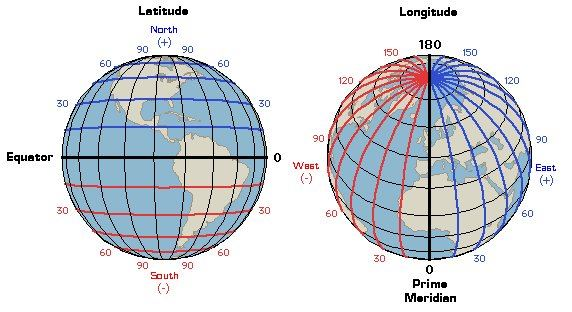
\includegraphics[width=1\textwidth]{figures/Latitude.jpg}}
	\caption{gambar Latitude.}
	\label{Gambar Latitude}
	\end{figure}
	garis khatulistiwa bumi, dan garis tengahnya adalah
	0, pusat bumi. Untuk menentukan latitude ( garis lintang ) dibeberapa titik P di permukaan, buatlah suatu jarak OP 
	ke suatu titik. Lalu sudut elevasi titik tersebut berada diatas garis ekuator adalah garis lintang l - lintang utara
	jika dari utara, lintang selatan ( negatif ) jika dari selatan. 
	Garis Lintang, dalam bola bumi, garis lintang dalam lingkaran memiliki perbedaan ukuran. Garis paling panjang adalah 
	Khatulistiwa, dimana yang lintangnya 0 ( nol ), sementara di daerah kutub, garis lintangnya 90° utara dan 90° selatan
	( atau bisa juga -90°) lingkarannya menyusut ke titik tertentu.

\section{BUJUR/LONGTITUDE}

	Longtitude adalah garis bujur, dimana garis bujur ini diawali dari titik 0° sampai 180° ke arah sebaliknya. Titik 0° dimulai dari
	garis negara Inggris, mengarah ke Indonesia akan menjadi angka positif. Jika koordinat longitude ( lintang ) akan menjadi minus 
	kearah kebalikan. Di bola bumi, garis bujur konstan meluas dari kutub ke kutub seperti batas segmen pada jeruk kupas. Garis Bujur atau
	Meridian ( gambar )
	\begin{figure}[ht]
	\centerline{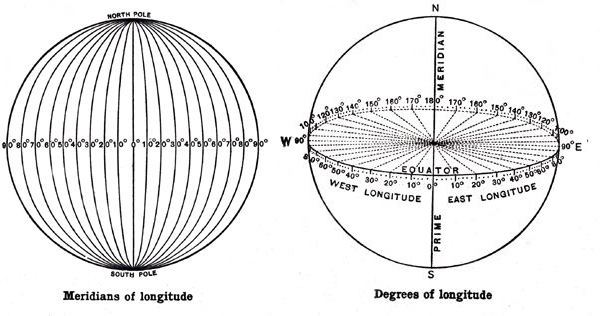
\includegraphics[width=1\textwidth]{figures/Longitude.jpg}}
	\caption{gambar longitude.}
	\label{Gambar Longitude}
	\end{figure}
	
	Setiap meridian harus menyberangi garis khatulistiwa. Karena khatulistiwa adalah sebuah lingkaran, kita bisa membagi nya seperti lingkaran
	yang lain ke dalam 360°,dan garis bujur f dari sebuah titik yang ditandai dimana meridian bertemu khatulistiwa.
	Nilai tersebut tentu bergantung pada saat kita mulai menghitung titik 0° garis bujur. Untuk alasan sejarah, garis bujur melewati Old Royal -
	Astronomical Obsevatory di Greenwich, Inggris, dimana garis 0° bujur di tetapkan. Berlokasi di tepi timur inggris, ibukota Inggris, Observatorium
	sekarang adalah Museum Umum dan suatu tanda yang membentang diatas halamannya yang menandai sebagai "garis meridian utama".
	Garis bujur atau dengan nama lain meridian, berasal dari bahasa latin, yaitu meri, variasi dari "merius" yang berarti "tengah" dan diem yang berarti 
	"hari". Kata tersebut juga bisa berarti "sore", dan waktu pada satu hari sebelum sore kita sebut sebagai "ante meridian" dimana waktu setelahnya berarti 
	"post meridian".Pada saat ini disingkat menjadi a.m. dan p.m. yang berasal dari istilah ini, dan matahari pada saat menjelang malam hari disebut sebagai
	"passing meridians". Semua titik pada setiap garis yang sama dalam garis bujur disebut sore ( dan pada jam lainnya ) pada saat yang sama dan oleh karena 
	itu disebut "garis meridian", yang menjadi "meridian" untuk lebih singkat.




%%%%%%%%%%%%%%%%%%%%%%%%%%%%%%%%%%%%%%%%%%%%%%%%%%%%%%
%% optional prologue or prologues
% \chapter{Chapter Title}
% \prologue{<text>}{<author attribution>}

%%%%%%%%%%%%%%%%%%%%%%%%%%%%%%%%%%%%%%%%%%%%%
% Edited Book: Author and Affiliation
%%%%%%%%%%%%%%%%%%%%%%%%%%%%%%%%%%%%%%%%%%%%%

% After \chapter{Chapter Title}, you can
% enter the author name and embed the affiliation with
% \chapterauthors{(author name, or names)
% \chapteraffil{(affiliation or affiliations)}
% }    

% For instance:
% \chapter{Chapter Title}
% \chapterauthors{G. Alvarez and R. K. Watts
% \chapteraffil{Carnegie Mellon University, Pittsburgh, Pennsylvania}

% For separate affiliations you can use \affilmark{(number)} after
% the name of a particular author and before the matching affiliation:

% For instance:
% \chapter{Chapter Title}
% \chapterauthors{George Smeal, Ph.D.\affilmark{1}, Sally Smith,
% M.D.\affilmark{2}, and Stanley Kubrick\affilmark{1}
% \chapteraffil{\affilmark{1}AT\&T Bell Laboratories
% Murray Hill, New Jersey\\
% \affilmark{2}Harvard Medical School,
% Boston, Massachusetts}
% }

%%%%%%%%%%%%%%%%%%%%%%%

%% short version of section head, or one without \\ supplied in sq. brackets.

% \section[Introduction and fugue]{Introduction\\ and fugue}
% \subsection[This is the subsection]{This is the\\ subsection}
% \subsubsection{This is the subsubsection}
% \paragraph{This is the paragraph}

% \begin{chapreferences}{widest label}
% \bibitem{<label>}Reference
% \end{chapreferences}

% optional chapter bibliography using BibTeX,
% must also have \usepackage{chapterbib} before \begin{document}
% Must use root file with \include{chap1}, \include{chap2} form.
%\bibliographystyle{plain}
%\bibliography{<your .bib file name>}

% optional appendix at the end of a chapter:
% \chapappendix{<chap appendix title>}
% \chapappendix{} % no title

%%%%%%%%%%%%%%%%%%%%%%%%%%%%%%%%%%%%%%%%%%%%%%%%%%%%%%%%%%%%%%%%
%% End Matter >>>>>>>>>>>>>>>>>>

% \appendix{<optional title for appendix at end of book>}
% \appendix{} % appendix without title

% \begin{references}{<widest label>}
% \bibitem{sampref}Here is reference.
% \end{references}

%%%%%%%%%%%%%%%%%%%%%%%%%%%%%%%%%%%%%%%%%%%%%%%%%%%%%%%%%%%%%%%%
%% Optional Problem Sets: Can use this at the end of each chapter or at end
%% of book

% \begin{problems}
% \prob
% text

% \prob
% text

% \subprob
% text

% \subprob
% text

% \prob
% text
% \end{problems}

%%%%%%%%%%%%%%%%%%%%%%%%%%%%%%%%%%%%%%%%%%%%%%%%%%%%%%%%%%%%%%%%
%% Optional Exercises: Can use this at the end of each chapter or at end
%% of book

% \begin{exercises}
% \exer
% text

% \exer
% text

% \subexer
% text

% \subexer
% text

% \exer
% text
% \end{exercises}

\bibliographystyle{IEEEtran}
\bibliography{aku,SejarahBumi,koordinatindo,definisi,longlat}
%%%%%%%%%%%%%%%%%%%%%%%%%%%%%%%%%%%%%%%%%%%%%%%%%%%%%%%%%%%%%%%%
%% INDEX: Use only one index command set:

%% 1) The default LaTeX Index
\printindex

%% 2) For Topic index and Author index:

% \usepackage{multind}
% \makeindex{topic}
% \makeindex{authors}
% \begin{document}
% ...
% add index terms to your book, ie,
% \index{topic}{A term to go to the topic index}
% \index{authors}{Put this author in the author index}

%% (these are Wiley commands)
%\multiprintindex{topic}{Topic index}
%\multiprintindex{authors}{Author index}

\end{document}

%%%%%%% Demo of section head containing sample macro:
%% To get a macro to expand correctly in a section head, with upper and
%% lower case math, put the definition and set the box 
%% before \begin{document}, so that when it appears in the 
%% table of contents it will also work:

\newcommand{\VT}[1]{\ensuremath{{V_{T#1}}}}

%% use a box to expand the macro before we put it into the section head:

\newbox\sectsavebox
\setbox\sectsavebox=\hbox{\boldmath\VT{xyz}}

%%%%%%%%%%%%%%%%% End Demo


Other commands, and notes on usage:

-----
Possible section head levels:
\section{Introduction}
\subsection{This is subsection}
\subsubsection{This is subsubsection}
\paragraph{This is the paragraph}

-----
Tables:
 Remember to use \centering for a small table and to start the table
 with \hline, use \hline underneath the column headers and at the end of 
 the table, i.e.,

\begin{table}[h]
\caption{Small Table}
\centering
\begin{tabular}{ccc}
\hline
one&two&three\\
\hline
C&D&E\\
\hline
\end{tabular}
\end{table}

For a table that expands to the width of the page, write

\begin{table}
\begin{tabular*}{\textwidth}{@{\extracolsep{\fill}}lcc}
\hline
....
\end{tabular*}
%% Sample table notes:
\begin{tablenotes}
$^a$Refs.~19 and 20.

$^b\kappa, \lambda>1$.
\end{tablenotes}
\end{table}

-----
Algorithm.
Maintains same fonts as text (as opposed to verbatim which uses fixed
width fonts). Space at beginning of line will be maintained if you
use \ at beginning of line.

\begin{algorithm}
{\bf state\_transition algorithm} $\{$
\        for each neuron $j\in\{0,1,\ldots,M-1\}$
\        $\{$   
\            calculate the weighted sum $S_j$ using Eq. (6);
\            if ($S_j>t_j$)
\                    $\{$turn ON neuron; $Y_1=+1\}$   
\            else if ($S_j<t_j$)
\                    $\{$turn OFF neuron; $Y_1=-1\}$   
\            else
\                    $\{$no change in neuron state; $y_j$ remains %
unchanged;$\}$ .
\        $\}$   
$\}$   
\end{algorithm}

-----
Sample quote:
\begin{quote}
quotation...
\end{quote}

-----
Listing samples

\begin{enumerate}
\item
This is the first item in the numbered list.

\item
This is the second item in the numbered list.
\end{enumerate}

\begin{itemize}
\item
This is the first item in the itemized list.

\item
This is the first item in the itemized list.
This is the first item in the itemized list.
This is the first item in the itemized list.
\end{itemize}

\begin{itemize}
\item[]
This is the first item in the itemized list.

\item[]
This is the first item in the itemized list.
This is the first item in the itemized list.
This is the first item in the itemized list.
\end{itemize}

%% Index commands
Author and Topic Indices, See docs.pdf and w-bksamp.pdf
